% mainfile: ../../main.tex
\chapter{Characterization and improvements of the optical path}\label{ch:setup:optics}
\AutoLettrine{Noise}

\section{Light coupling}\label{sec:setup:optics:coupling}
\Glspl{smf} are a natural choice to transmit laser light which usually consists of a just that, a single mode.
Because the mode profile of \glspl{smf} is very close to the fundamental laser mode, \acrshort{tem}$_{00}$, \emph{Gaussian optics} are required to describe the propagating light.

\begin{enumerate}
    \item Gaussian optics equations \begin{enumerate}
        \item electric field profile
        \item rayleigh length
        \item beam divergence \& diameter
    \end{enumerate}
    \item diffraction limit
    \item \gls{na}
    \item beam diameter
    \item choosing lenses
\end{enumerate}

\subsection{Light collection}\label{sec:setup:optics:coupling:detection}
In a confocal microscope geometry, light is collected using the same lens that is also used for illumination of the sample.
For excitation with a Gaussian laser beam but non-Gaussian radiation profiles being emitted, this means that two different beam behaviors need to be matched, a task that is likely not going to be possible to achieve completely.
% The SMF character is crucial for excitation rejection
Since furthermore the emitted light is coupled into a \gls{smf}, losses will invariably occur when focusing the non-Gaussian beam onto the \gls{smf} acting as a spatial filter.
A detailed analysis of the electric field profile to compute the expected coupling efficiency from the sample into the \gls{smf} is beyond our scope here.
It would require taking into account the full sample and lens geometries as well as diffraction, a task only possible by employing a full-fledged numerical optics simulation suite.
However, we can make some crude simplifications of the problem to estimate the order of magnitude of these effects.
To this end, I model the light source as a point dipole beneath the surface of a homogeneous slab of dielectric material and the real lenses as ideal thin lenses.
% TODO: Argue why dipole
%Inside the semiconductor, optical interband transitions are well described by in-plane dipole matrix elements~\cite{Gu2013}.
% TODO: maybe a book reference here instead
%Address crude approximations, mention more rigorous approach with some proper optical simulation software.

\begin{marginfigure}
    \begin{tikzpicture}[
    scale=2,%
    font=\footnotesize,%
    thick,%
    axis/.style={RWTHblack75,text=black},%
]
    % requires libraries angle,quotes,calc

    \newlength\CA
    \setlength\CA{1cm}
    \newlength\tick
    \setlength\tick{0.1cm}

    \coordinate (origin) at (0,0);
    \coordinate (dipole) at (0,-0.5);
    \coordinate (interfacemargin) at (0.25,0);
    \coordinate (lens) at (0,1);
    \coordinate (lensmargin) at ($(\CA,1)$);

    % Coordinate axes
    \draw[->,axis]
        (origin)
        -- ($(\CA,0) + (0.4,0)$) node[right] {$x$}
    ;
    \draw[->,axis]
        (0.0,-0.75)
        -- ($(lens) + (0,0.25)$) node[above] {$z$}
    ;
    % Xticks
    \draw[axis]
        (\CA,0)
        -- ++(0,-\tick) node[below] {$w$}
    ;
    % Yticks
    \draw[axis]
        (lens)
        -- ++(-\tick,0) node[left] {\fob}
        (origin)
        -- ++(-\tick,0) node[left] {$0$}
        (dipole)
        -- ++(-\tick,0) node[left] {$-d$}
    ;
    % Angles
    \draw[thin,axis]
        ($(interfacemargin) - (0,0.1)$)
        -- ++(0,0.5) node (beta) {}
    ;
    \pic[draw,"$\alpha$",angle eccentricity=1.5,axis]
        {angle = interfacemargin--dipole--origin}
    ;
    \pic[draw,"$\beta$",angle eccentricity=1.5,axis]
        {angle = lensmargin--interfacemargin--beta}
    ;

    % Lens and QW
    \draw[very thick]
        (lens)
        -- ++(1.25,0) node[right] {Ob.}
    ;
    \draw[dashed,RWTHblack75]
        ($(dipole) + (0,0.05)$)
        -- ++(1.25,0)
        ($(dipole) - (0,0.05)$)
        -- ++(1.25,0)
    ;
    \node[anchor=west] at ($(dipole) + (1.25,0)$) {\acrshort{qw}};

    % Margin beam
    \draw[->,RWTHred100]
        (dipole)
        -- (interfacemargin)
        -- (lensmargin)
        -- ++(0,0.25)
    ;
\end{tikzpicture}

    \caption[\imgsource{img/tikz/setup/emission.tex}]{
        Sketch of a light source located inside a dielectric medium ($z < 0, n > 1$) emitting light in the upwards direction to collection by an objective lens in air ($z > 0, n = 1$).
        The red line indicates the marginal ray of the lens with focal length \fob and \gls{ca} $2w$.
    }
    \label{fig:setup:optics:coupling:emission}
\end{marginfigure}

Consider the situation sketched in \cref{fig:setup:optics:coupling:emission}.
A dipole oriented along $x$ in the plane of a \ch{GaAs} \gls{qw} with refractive index $n$ buried at a depth $d$ beneath the surface of the sample emits light into the halfspace above it.
The emitted radiation has the electric field distribution
\begin{equation}\label{eq:setup:optics:coupling:efield}
    E(x,y,z) = E_{0}\frac{\exp(\i k r)}{r}\cos\theta
\end{equation}
where $\theta=\arctan{\flatfrac{x}{z}}$, $r$ is the distance from the point dipole and $k=\flatfrac{2\pi}{\lambda}=\flatfrac{2\pi n}{\lambda_0}$ is the wavenumber in the medium.

The emitted light is refracted at the surface and we collect and collimate it with an objective lens (labelled \enquote{Ob.}) with $\mr{\acrshort{na}}=\sin\theta^\prime_\mr{m}$ at distance \fob above the surface of the sample, where \fob is the focal length and $\theta^\prime_\mr{m}$ the angle of the marginal ray.
The \gls{na} determines the maximum amount of light the objective lens can collect, and using Snell's law we can relate the angle of a ray outside the sample $\theta^\prime$ to the angle inside the sample $\theta$,
\begin{equation}\label{eq:setup:optics:coupling:snell}
    \sin\theta^\prime = n\sin\theta,
\end{equation}
with $n\approx 3.57$ at $\lambda_0=\qty{800}{\nano\meter}$ and $T=\qty{0}{\kelvin}$.
This yields $\theta_{\mr{m}} = \arcsin(\flatfrac{\mr{\acrshort{na}}}{n}) \approx\qty{11}{\degree}$ for the emission angle of the marginal ray inside the semiconductor, suggesting that \cref{eq:setup:optics:coupling:efield} is well approximated as a spherical wave since $\cos\theta_{\mr{m}}\approx 1-\theta_{\mr{m}}^2/2\approx 1$.
Indeed, the fraction of the emitted intensity $I(\theta)\propto\abs{E(\theta)}^2$ being collected by the objective lens, the \emph{collection efficiency}, is
\begin{equation}\label{eq:setup:optics:coupling:efficiency:collection}
\begin{split}
    \eta_{\mr{c}} &= \frac{\iint_{\theta_{\mr{m}}}\dd{\Omega} I(\theta)}{\iint\dd{\Omega} I(\theta)} \\
                  &= \frac{\int_{0}^{\theta_{\mr{m}}}\dd{\theta}\sin\theta\cos^2\theta}{\int_{0}^{\pi}\dd{\theta}\sin\theta\cos^2\theta} \\
                  &= \frac{1}{2}\left(1 - \left[1 - \left(\frac{\mr{\acrshort{na}}}{n}\right)^2\right]^{\flatfrac{3}{2}}\right)
\end{split}
\end{equation}
which evaluates to only $\eta_{\mr{c}}\approx\qty{2.8}{\percent}$ for the objective lens's $\mr{\acrshort{na}}=\num{0.7}$.
Moreover, since $d\sim\qty{100}{\nano\meter}\ll\fob\sim\qty{1}{\milli\meter}$ and also $kd\ll 1$, the lateral extent of the light source as viewed from the objective lens is negligibly small and is well approximated by a point source right below the surface.\sidenote{
    Note that I use $f = \flatfrac{\mr{\acrshort{ca}}}{2\mr{\acrshort{na}}}$ rather than the effective focal length quoted by the manufacturer in this section.
}

In order to determine the electric field amplitude as a function of position inside the lens with radius $w$, consider a light ray impinging on the surface at lateral position $x_0$.
Taking two points of the light ray at $(x_0-\Delta x, -\epsilon)$ some $\epsilon > 0$ below the surface and $(x_0 + \Delta x^\prime, +\epsilon)$ above, we can express the lateral shift due to refraction as
\begin{equation}
    \Delta x^{\prime} = \epsilon\tan\theta^{\prime} = \Delta x \frac{n\cos\theta}{\sqrt{1 - n^2\sin^2\theta}}
\end{equation}
with $\theta^{(\prime)} = \arctan(\Delta x^{(\prime)}/\epsilon)$ using standard trigonometric identities.
Thus, the coordinate $x$ of the electric field inside the semiconductor transforms to the coordinate $x^\prime$ outside the semiconductor as
\begin{equation}
    x\to x^{\prime} = x n \left[1 + \left(\frac{x}{z}\right)^2 - \left(\frac{nx}{z}\right)^2\right]^{-\frac{1}{2}},
\end{equation}
which we invert to obtain
\begin{equation}\label{eq:setup:optics:coupling:coordinate_trafo}
    x = \frac{z}{\sqrt{n^2\left[1 + (z/x^{\prime})^2\right] - 1}}.
\end{equation}

We now approximate the light source as a point source at $z=-\epsilon < 0$ emitting a spherical wave as discussed above and introduce cylindrical coordinates with $\rho^{\prime} = \sqrt{x^{\prime 2} + y^2}$ so that $r = \sqrt{\rho^{\prime 2} + z^2}$.
Plugging \cref{eq:setup:optics:coupling:coordinate_trafo} into \cref{eq:setup:optics:coupling:efield} then yields
\begin{equation}\label{eq:setup:optics:coupling:efield:lens}
    E(\rho^\prime,z) = E_0\frac{\exp(\i k z\zeta(\rho^{\prime}))}{z\zeta(\rho^{\prime})}
\end{equation}
with
\begin{equation}
    \zeta(\rho^{\prime}) = \sqrt{1 + \left(n^2\left[1 + (z/\rho^{\prime})^2\right] - 1\right)\inverse}
\end{equation}
for the electric field outside the semiconductor.
At the lens $\zeta\approx 1$ so that the field is actually more closely resembled by a plane rather than the original spherical wave.

\begin{marginfigure}
    \centering
    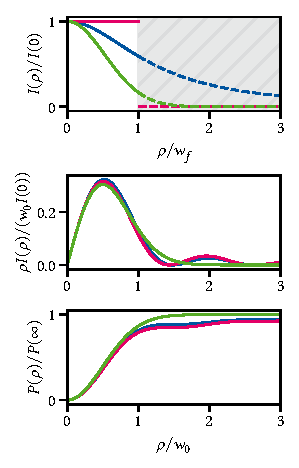
\includegraphics{img/pdf/setup/modes_1d}
    \caption[\imgsource{img/py/setup/single_mode_fiber_coupling.py}]{
        Electric field modes.
        Top: mode intensity of the light collected from the semiconductor at the objective lens plane (blue) in comparison to a flattop (green) and Gaussian \acrshort{tem}$_{00}$ mode with theoretical beam diameter after collimating with the ocular lens.
        $w$ is the lens \gls{ca} radius.
        Middle: diffraction pattern of the collimated beam approximated as a flattop when focusing onto the \gls{smf} end face with the ocular lens (green) and the fiber's guiding mode (magenta).
        The curves are scaled with the radial coordinate $\rho$ to highlight the Airy rings.
        Bottom: power encased by a circle with radius $\rho$, $P(\rho)\propto\int_0^{\rho}\dd{\rho^\prime} \rho^{\prime} I(\rho^{\prime})$.
    }
    \label{fig:setup:optics:coupling:modes_1d}
\end{marginfigure}

The radial intensity profile given by the absolute value square of \cref{eq:setup:optics:coupling:efield:lens} is shown in the upper panel of \cref{fig:setup:optics:coupling:modes_1d} together with a flattop (green) and a Gaussian (magenta) beam profile for comparison.
The intensity drops only by about \qty{2}{\percent} at the edge of the lens aperture, $\rho=w$.
We may thus expect non-negligible loss when coupling this beam into a \gls{smf} with a guiding mode very closely approximating the Gaussian \acrshort{tem}$_{00}$ mode~\cite{Yariv1989,Kowalevicz2006}
\begin{equation}\label{eq:setup:optics:coupling:efield:tem00}
    E(\rho, z) = E_0\frac{w_0}{w(z)}\exp\left\lbrace -\i\left[kz - \arctan(\frac{z}{z_0})\right] - \rho^2\left[\frac{1}{w(z)^2} + \frac{ik}{2 R(z)}\right]\right\rbrace
\end{equation}
with the fiber's \gls{mfd} $2 w_0$, the beam's $1/\e$-radius
\begin{equation}
    w(z)^2 = w_0^2\left(1 + \frac{z^2}{z_0^2}\right),
\end{equation}
the wavefront radius of curvature
\begin{equation}
    R(z) = z\left(1 + \frac{z_0^2}{z^2}\right),
\end{equation}
the Rayleigh range
\begin{equation}
    z_0 = \frac{\pi w_0^2 n}{\lambda},
\end{equation}
and where $z=0$ in the fiber end face.

The light collected and collimated by the objective lens next passes through the ocular lens in the detection arm which focuses it into the \gls{smf}.
The image of the beam on the fiber end face is given by the Fraunhofer diffraction pattern generated by the (approximately) plane wave incident on the ocular lens aperture,\sidenote{
    We can safely neglect diffraction effects from the objective lens aperture.
    The Fraunhofer criterion $\flatfrac{b^2}{\lambda}$ with $b$ the aperture diameter is $\approx\qty{30}{\meter}$, implying the ocular lens at a distance of $\sim\qty{1}{\meter}$ is in the near field with many Fresnel zones where diffraction does not yet play a significant role~\cite{Hecht2017}.
}
resulting in the Airy disk~\cite{Hecht2017}
\begin{equation}\label{eq:setup:optics:coupling:airy}
    E(q) = E_0 2\pi w^2\frac{\exp(\i k \foc)}{\foc} \frac{J_1(\flatfrac{kwq}{\foc})}{\flatfrac{kwq}{\foc}},
\end{equation}
where $J_1(x)$ is Bessel function of order one and $q$ the radial coordinate in the image plane, \ie, the fiber end face.
\Cref{eq:setup:optics:coupling:airy} scaled with the radius $\rho$ is plotted in the middle panel of \cref{fig:setup:optics:coupling:modes_1d} together with the \gls{smf}'s guiding Gaussian mode.
While within the \gls{mfd} the two modes match quite well, a relevant amount of the power $P(\rho)\propto \int_0^{\rho}\dd{\rho^{\prime}} \rho^{\prime} I(\rho^{\prime})$ resides outside that radius as shown in the bottom panel of the same figure.

The mode matching efficiency is then given by the normalized spatial overlap of the light field ($E_{\mr{l}}$, \cref{eq:setup:optics:coupling:efield:lens}) and the fiber's guiding mode ($E_{\mr{f}}$, \cref{eq:setup:optics:coupling:efield:tem00})~\cite{Paschotta2005},
\begin{equation}\label{eq:setup:optics:coupling:efficiency:mode_matching}
    \eta_{\mr{m}} = \frac{\int\dd{S}\abs{E_{\mr{f}}(\rho)}^2\int\dd{S}\abs{E_{\mr{l}}(\rho)}^2}{\abs{\int\dd{S} E_{\mr{f}}(\rho) E_{\mr{l}}(\rho)}^2} \approx\qty{77}{\percent}
\end{equation}
for our parameters.

